\begin{section}{Metodologia}
\subsection{Prepara��o do Servidor}
O servidor, por ser o elemento chave na consolida��o do projeto, deve ser o 
m�dulo a ser prioritariamente configurado, a fim de ser preparado para atender
�s devidas requisi��es, bem como executar qualquer tipo de aplica��o solicitada.
Sendo assim, a instala��o da plataforma �ngstr\"{o}m foi tomada como o primeiro
passo. �ngstr\"{o}m~\cite{angstrom} � um sistema operacional, baseado em Linux,
preparado exclusivamente para plataformas embarcadas, sendo o padr�o para a 
pr�pria BeagleBone.

\subsection{Reconhecimento de Voz}
% http://eda.eme.ro/handle/10598/28187
Em~\cite{cassio14}, o Julius foi configurado para funcionar em modo servidor
atrav�s da op��o nativa ``-adinnet'' (A/D \textit{Input from Network}, convers�o 
A/D com entrada pela rede). Isso permite que o Julius receba amostras de �udio
via \textit{streaming} atrav�s de uma comunica��o com um cliente gen�rico via
\textit{socket}.

\subsection{S�ntese de Voz}
% http://stackoverflow.com/questions/2661129/espeak-sapi-dll-usage-on-windows

\subsection{Servidor LAMP}

\subsection{Cliente Android}
Tamb�m em~\cite{cassio14}, 

\begin{figure}[!h]
	\centering
	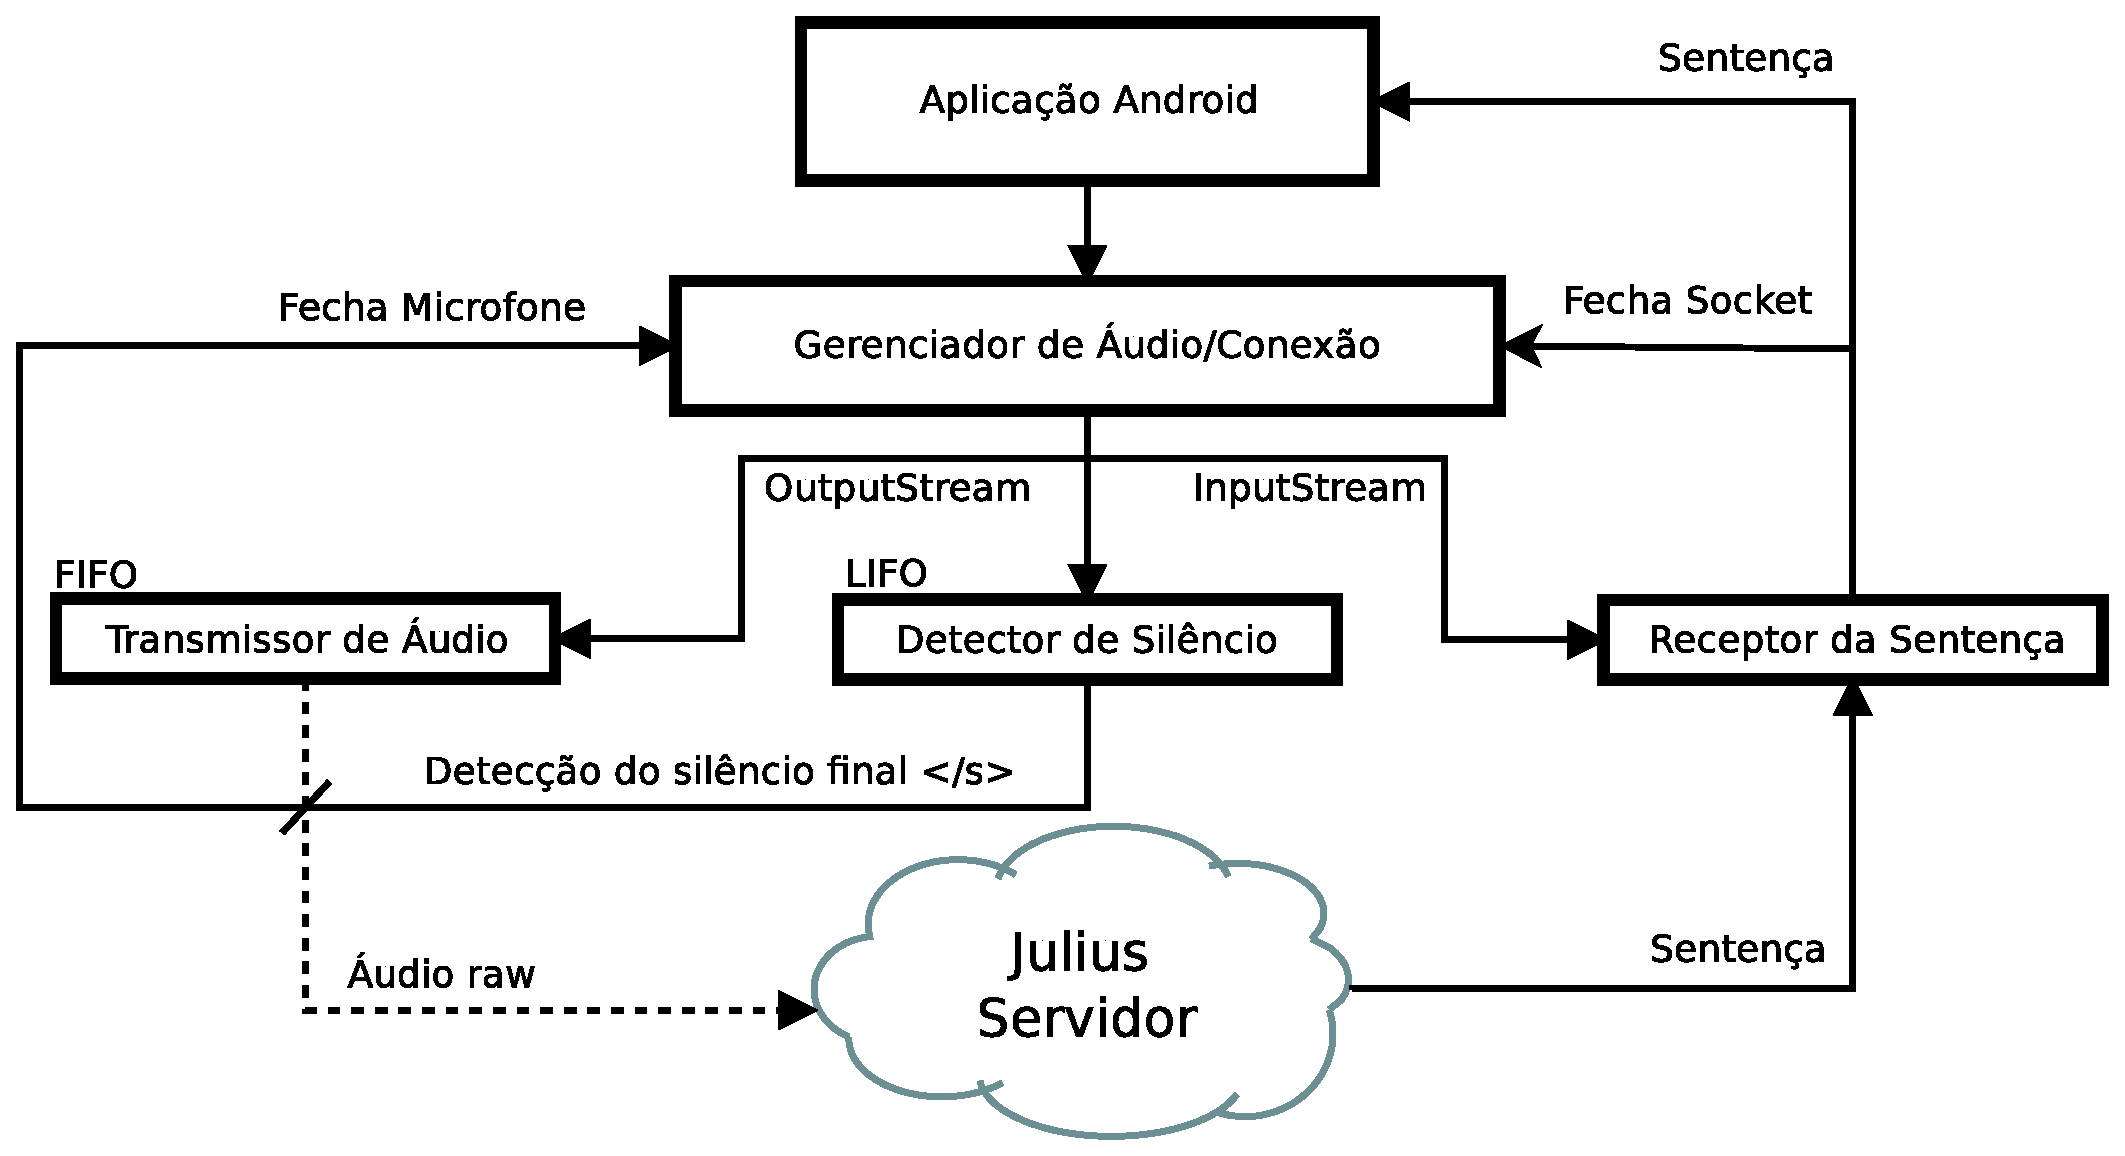
\includegraphics[width=.90\textwidth]{Figures/csr}
	\caption{Esquem�tico do Cliente LaPS CSR.}
	\label{fig:asr_sch}
\end{figure}

\end{section}
